% 06-language-model-exploration.tex

% Language Models Exploration
% 6.1. Introduction: Provides an overview of the language models task and its objectives.
% 6.2. Pretraining: Describes the process of pretraining Doc2Vec or using a pretrained Bert model.
% 6.3. Model Fine-tuning: Fine-tunes the last layer of the network.
% 6.4. Learning Curves: Plots learning curves and determines the optimal number of epochs.

% Section Title
\section{LANGUAGE MODEL EXPLORATION}

    % Main Content

    \subsection{Introduction}
    
        This section documents the steps taken to fine-tune a pre-trained BERT model for multi-label classification.
        The focus was on customizing the final classification layer and training the model on the \cooltext{Set\_Fingerprint} intents. Performance metrics and visualizations are presented to evaluate the effectiveness of the model.

    \subsection{Data Preprocessing}

        The dataset was processed as follows:

        \begin{itemize}

            \item The \cooltext{full\_session} column, which contains lists of words, was filtered to retain only words that appeared at least in 1\% of all the sessions. This step reduced the vocabulary to frequent words only.

            \item The \cooltext{Set\_Fingerprint} column was preprocessed for multi-label encoding using the \cooltext{MultiLabelBinarizer} class, enabling the representation of intents as binary vectors.

            \item The dataset was split into 60\% training, 20\% validation, and 20\% testing sets.
        \end{itemize}

    \subsection{Tokenization}

        The tokenization process is a critical step in preparing text data for input into a BERT model. We utilized the pre-trained BERT tokenizer, specifically designed for the \cooltext{bert-base-uncased} model, to convert our text data into input IDs and attention masks. Using the pre-trained tokenizer ensures consistency with BERT's pre-training, maintaining representation integrity and optimizing model performance. These strategies enhance efficiency, compatibility, and overall performance in the text processing pipeline.

    \subsection{Model Architecture}

        A pre-trained \cooltext{bert-base-uncased} model was used, with a custom linear classification head added to predict the intents. The classifier had an input size of 768 (BERT's hidden layer dimensions) and an output size equal to the number of intents. The model architecture is as follows:

        \begin{itemize}
        
            \item \cooltext{CustomBERTModel}: A custom model class that inherits from \cooltext{torch.nn.Module}.
            \item \cooltext{BertModel}: The pre-trained BERT model.
            \item \cooltext{classifier}: A dense layer with a sigmoid activation function that maps the BERT output to the number of intents.
        
        \end{itemize}
        
        The choice of a dense layer with sigmoid activation is motivated by the multi-label nature of our classification task. In multi-label classification, each instance can be associated with multiple labels simultaneously. The sigmoid activation allows each output neuron to independently predict the probability of its corresponding intent being present, which is essential for handling non-mutually exclusive labels.

    \subsection{Training Process}

        \begin{itemize}
        
            \item The model was trained using the AdamW optimizer with a learning rate of $4 \times 10^{-5}$, betas of (0.9, 0.98), and an epsilon of $1 \times 10^{-6}$.

            \item A linear learning rate scheduler was used with no warmup steps and a total of \cooltext{num\_training\_steps} steps.

            \item The \cooltext{BCEWithLogitsLoss} loss function was applied for multi-label classification.

            \item The model was fine-tuned for 4 epochs, with a batch size of 16. Specifically, only the last layer (the custom classification head) was trained, while the pre-trained BERT layers were kept frozen. 
            
        \end{itemize}

        \subsection{Evaluation Metrics}

        \begin{itemize}
        
            \item Metrics included precision, recall, F1-score, and ROC-AUC for each intent class.

            \item ROC curves were generated for each class to visualize the trade-off between true positive rate and false positive rate.

            \item Training and validation loss curves were plotted to monitor the model's learning progress over epochs.
            
        \end{itemize}
        

    \subsection{Results}

        \subsubsection{Training and Validation Loss \\}

            The training and validation loss curves shown in Figure~\ref{fig:loss} indicate a consistent decrease in both losses over the epochs, suggesting that the model is learning effectively. The training loss and validation loss both trend downwards, with no significant signs of overfitting, as the validation loss does not increase while the training loss decreases. This convergence implies that the model generalizes well to the validation data.
            
            However, it is important to note that while the losses show a consistent decrease, we do not know for how much longer this trend could continue. The optimal number of epochs remains unclear, as we stopped training after 4 epochs due to resource constraints. Further experimentation with additional epochs could provide deeper insights into the model's learning dynamics and potentially improve performance. 
            
            \begin{figure}[h]
                \centering
                \begin{minipage}[c]{0.47\textwidth}
                    \centering
                    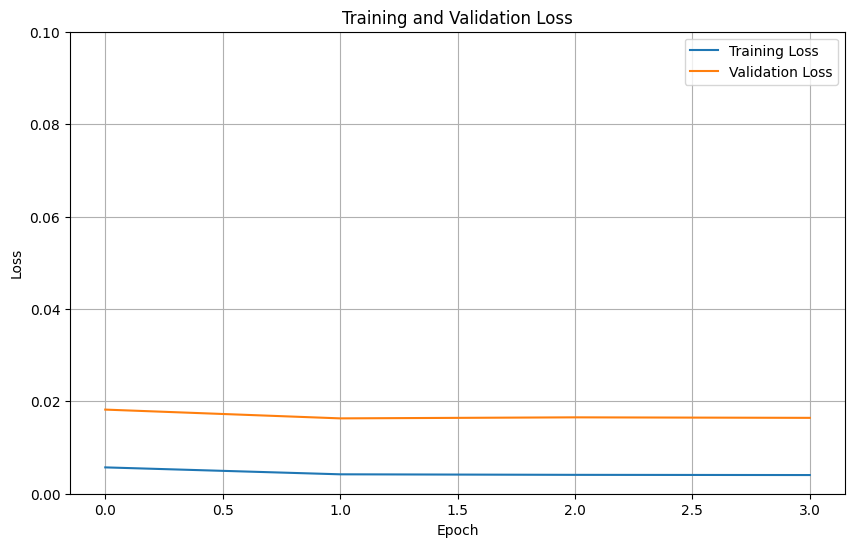
\includegraphics[width=\textwidth]{../figures/plots/section4/loss_curves.png}
                    \caption{Training and Validation Loss}
                    \label{fig:loss}
                \end{minipage}
                \hfill
                \begin{minipage}[c]{0.47\textwidth}
                    \centering
                    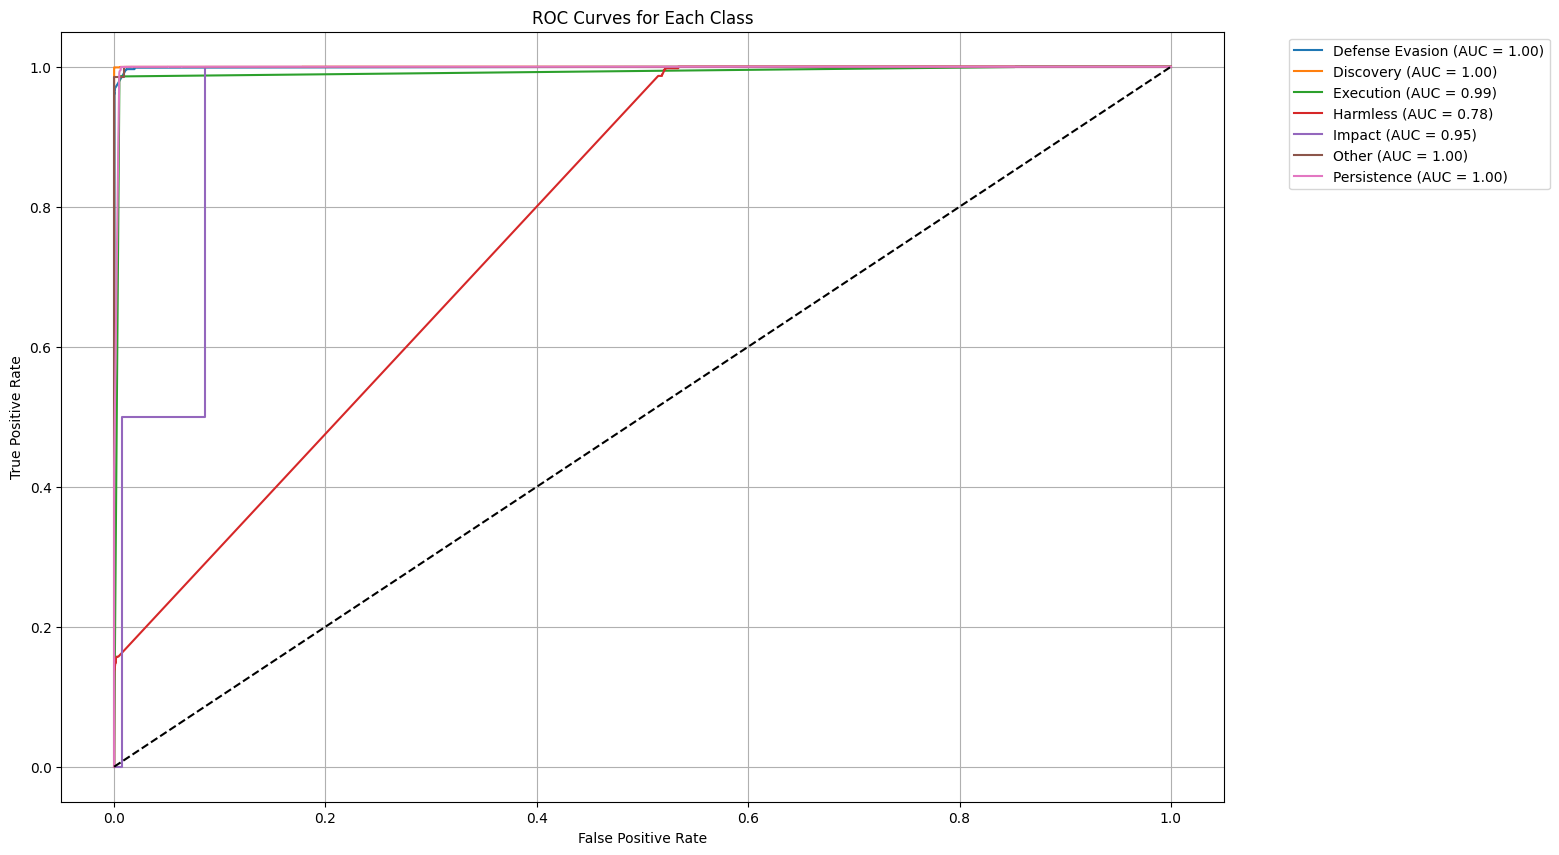
\includegraphics[width=\textwidth]{../figures/plots/section4/roc_curves.png}
                    \caption{ROC Curves for Each Class}
                    \label{fig:roc}
                \end{minipage}
            \end{figure}

        \subsubsection{ROC Curves \\}

            The ROC curves for each class, as depicted in Figure~\ref{fig:roc}, show excellent performance for most classes, with AUC values close to 1.00 for Defense Evasion, Discovery, Execution, Other, and Persistence. Notably, the Harmless class has a lower AUC of 0.78, indicating potential difficulties in distinguishing this class from others. This could suggest class imbalance or other challenges specific to identifying harmless intents.
            
        \subsubsection{Test Metrics \\}
        
            The model achieved the following high weighted metrics on the test set:
            
            \begin{itemize}
                \item Precision: 0.9974
                \item Recall: 0.9927
                \item F1-Score: 0.9937
                \item ROC-AUC: 0.9971
            \end{itemize}
            
            These weighted metrics indicate superior performance, capturing most positive cases accurately while accounting for class imbalance. 
            
    \subsection{Conclusion}

        The BERT-based model demonstrated exceptional performance in classifying SSH attack sessions into MITRE ATT\&CK tactics, achieving high precision, recall, F1-score, and ROC-AUC values. Notably, the model excelled in identifying malicious intents, as evidenced by the high AUC values for classes such as Defense Evasion and Persistence. However, the "Harmless" class presented challenges, indicating potential issues with class imbalance and feature representation.

        Several factors contribute to these findings. The limited number of examples for harmless activities may have hindered the model's ability to learn distinguishing features effectively. Future research could explore fine-tuning more layers of the BERT model to enhance performance, or adding more instances and sessions of the lesser classes, making the dataset more balanced. Additionally, feature engineering and exploring different architectures could improve the model's discriminative power.

        In summary, this study contributes to the field by successfully applying a BERT-based model to classify SSH attack sessions, achieving high performance, and identifying areas for improvement. The insights gained suggest promising directions for enhancing the model's capabilities in distinguishing harmful from harmless intents, thereby advancing cybersecurity defenses.
